\section{Variation of settings of the networked SEIR model identification and simulation}\label{sec:variationsOfSEIRSettings}
This section presents the impact of different time ranges on the results of the parameter identification and subsequent simulation. To provide a better understanding of the effects of the options on the behavior of the networked SEIR model, both the aggregated, denormalized compartment levels and the normalized compartment levels per county are presented. As can be seen, aggregated levels are more consistent with the real pandemic activity, while the spread levels of the individual counties show large deviations resulting from this work's focus on the mobility behavior of the population and suggesting to consider additional data for the scaling factors $\psi$.

\subsection{Wave 1 - from 01-FEB-2020 to 01-SEP-2020}

\autoref{fig:compCombWave1} shows how the networked SEIR model fails to recover the spread activity for wave 1. The root cause is unknown, but indicates, that mobility is only one of the many drivers of a pandemic.

\begin{figure}[hbtp]
     \centering
     \begin{subfigure}[b]{.45\linewidth}
         \centering
         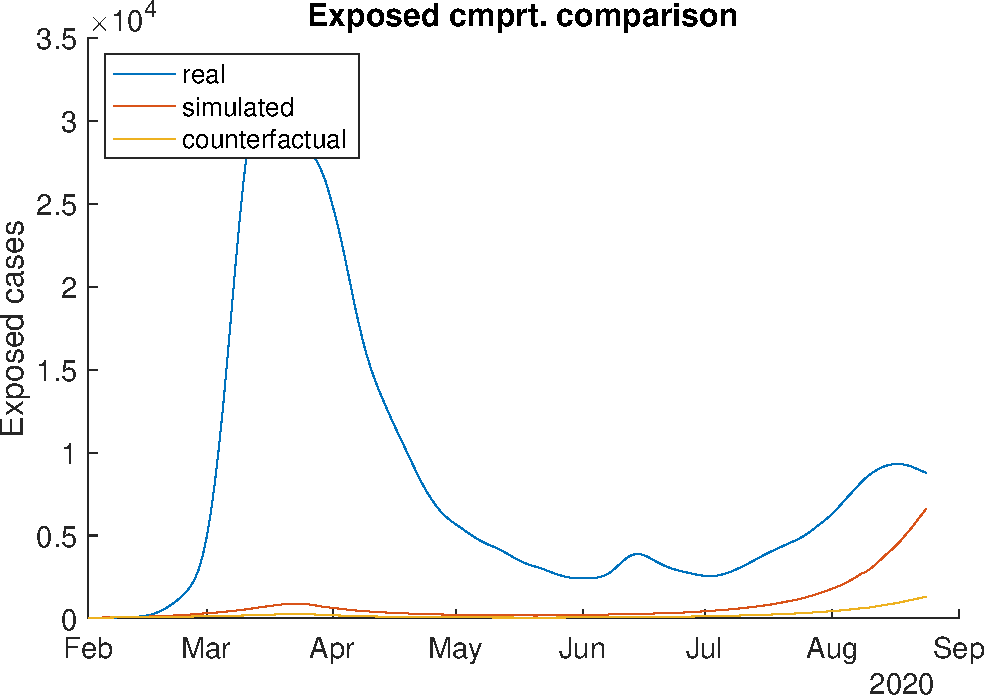
\includegraphics[width=\linewidth]{img/210907_221615_combined_wave1/figures/COMP_exp}
         \caption{Exposed}
         \label{fig:compAggrCombWave1Exp}
     \end{subfigure}
     \hfill
     \begin{subfigure}[b]{.45\linewidth}
         \centering
         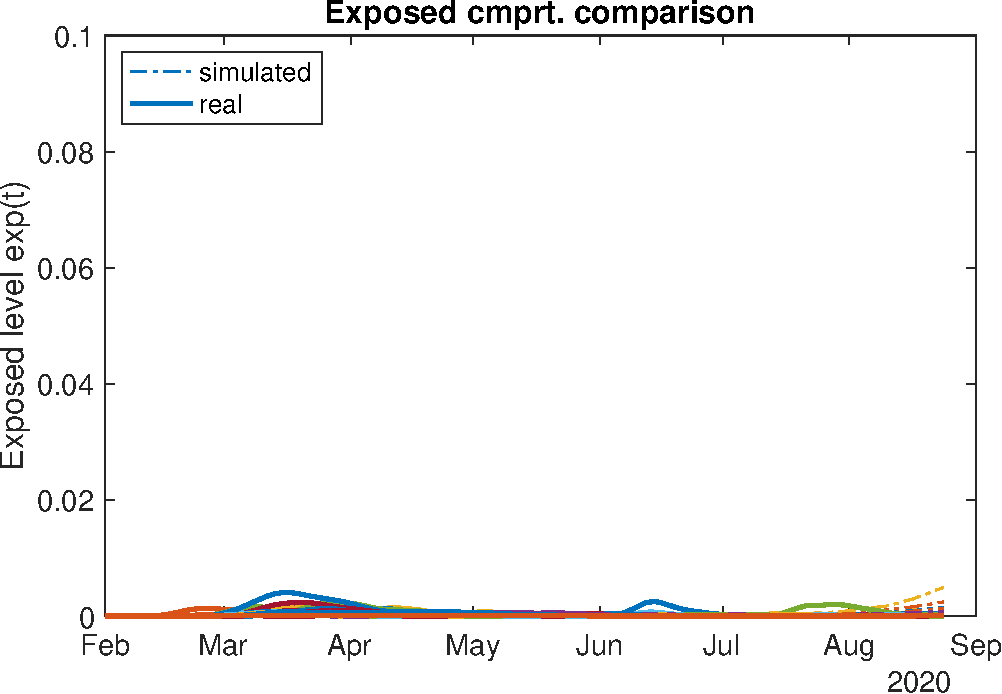
\includegraphics[width=\linewidth]{img/210907_221615_combined_wave1/figures/SEIR_e_sim-vs-real}
         \caption{Exposed}
         \label{fig:compCombWave1Exp}
     \end{subfigure}
     \newline
     \begin{subfigure}[b]{.45\linewidth}
         \centering
         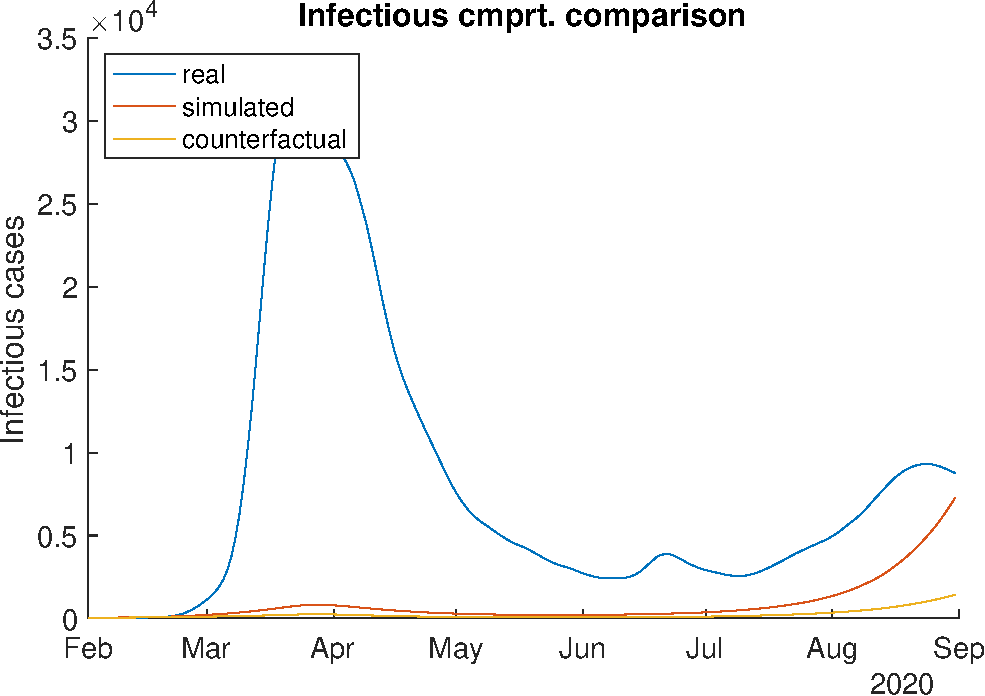
\includegraphics[width=\linewidth]{img/210907_221615_combined_wave1/figures/COMP_inf}
         \caption{Infectious}
         \label{fig:compAggrCombWave1Inf}
     \end{subfigure}
     \hfill
     \begin{subfigure}[b]{.45\linewidth}
         \centering
         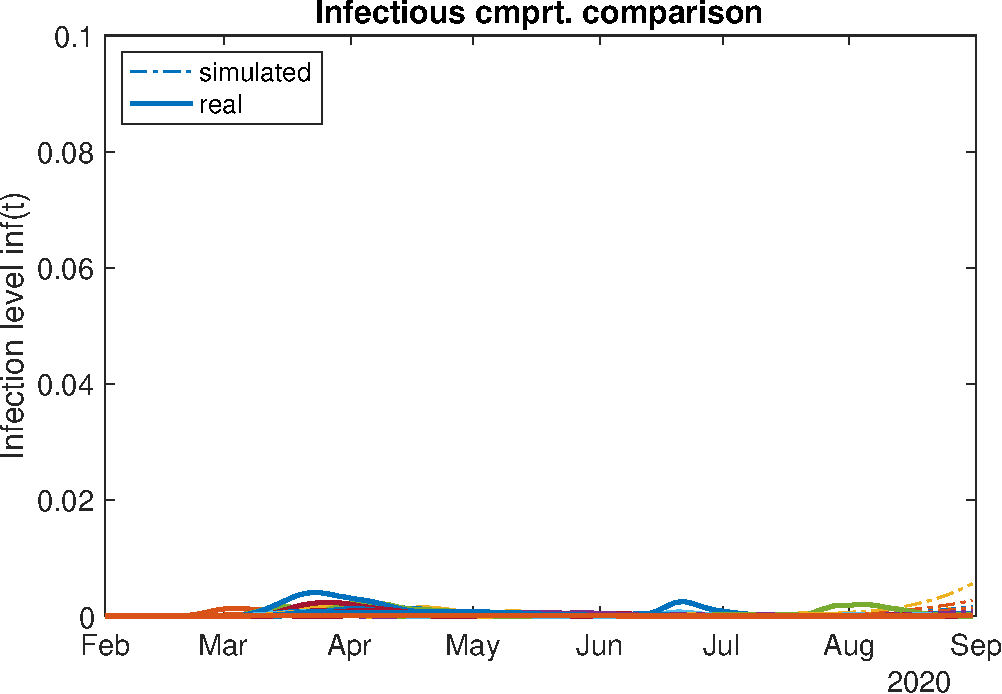
\includegraphics[width=\linewidth]{img/210907_221615_combined_wave1/figures/SEIR_i_sim-vs-real}
         \caption{Infectious}
         \label{fig:compCombWave1Inf}
     \end{subfigure}
     \newline
     \begin{subfigure}[b]{.45\linewidth}
         \centering
         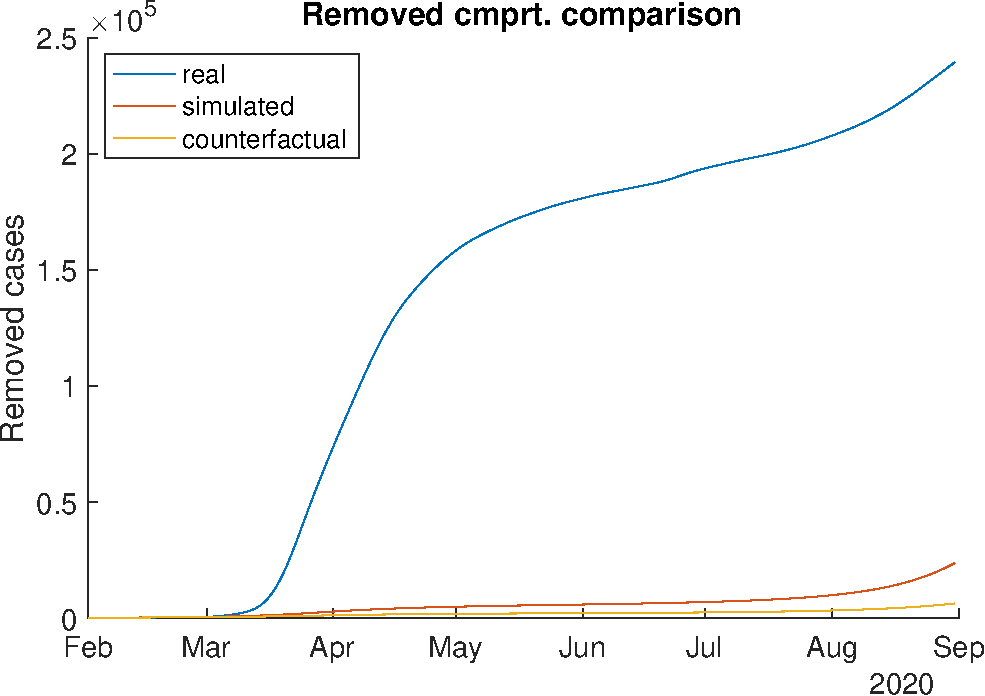
\includegraphics[width=\linewidth]{img/210907_221615_combined_wave1/figures/COMP_rem}
         \caption{Removed}
         \label{fig:compAggrCombWave1Rem}
     \end{subfigure}
     \hfill
     \begin{subfigure}[b]{.45\linewidth}
         \centering
         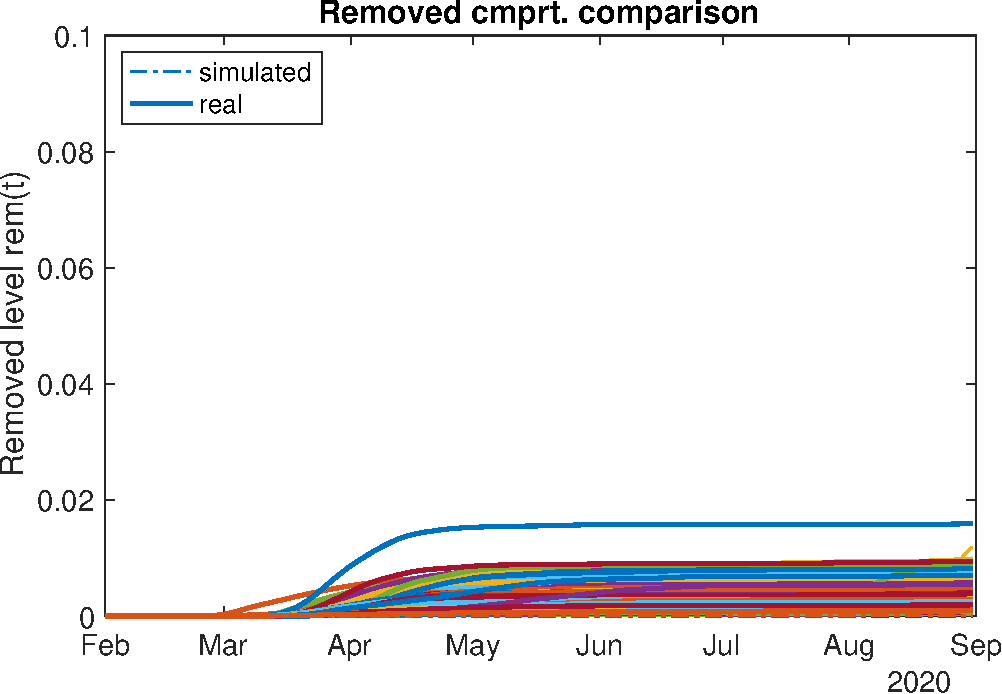
\includegraphics[width=\linewidth]{img/210907_221615_combined_wave1/figures/SEIR_r_sim-vs-real}
         \caption{Removed}
         \label{fig:compCombWave1Rem}
     \end{subfigure}     
     \caption{Compartment levels, wave 1 with combined mobility; left: normalized per county, right: aggregated denormalized}
     \label{fig:compCombWave1}
\end{figure}

\subsection{Wave 2 - from 01-SEP-2020 to 15-MAR-2021}

\autoref{fig:compCombWave2} is a good example of the performance of the networked SEIR model. As can be seen, the simulated behavior is matching the real behavior both in time and magnitude of the outbreak. The counterfactual shows similar reduction in pandemic activity as was shown for the complete time period in \autoref{sec:evaluation}.

\begin{figure}[hbtp]
     \centering
     \begin{subfigure}[b]{.45\linewidth}
         \centering
         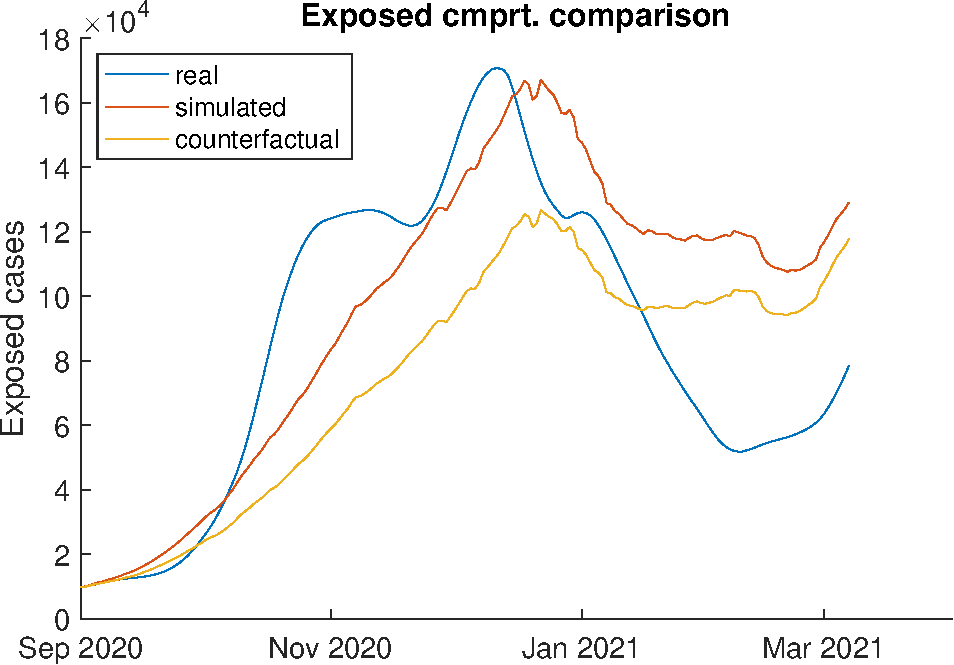
\includegraphics[width=\linewidth]{img/210907_223108_combined_wave2/figures/COMP_exp}
         \caption{Exposed}
         \label{fig:compAggrCombWave2Exp}
     \end{subfigure}
     \hfill
     \begin{subfigure}[b]{.45\linewidth}
         \centering
         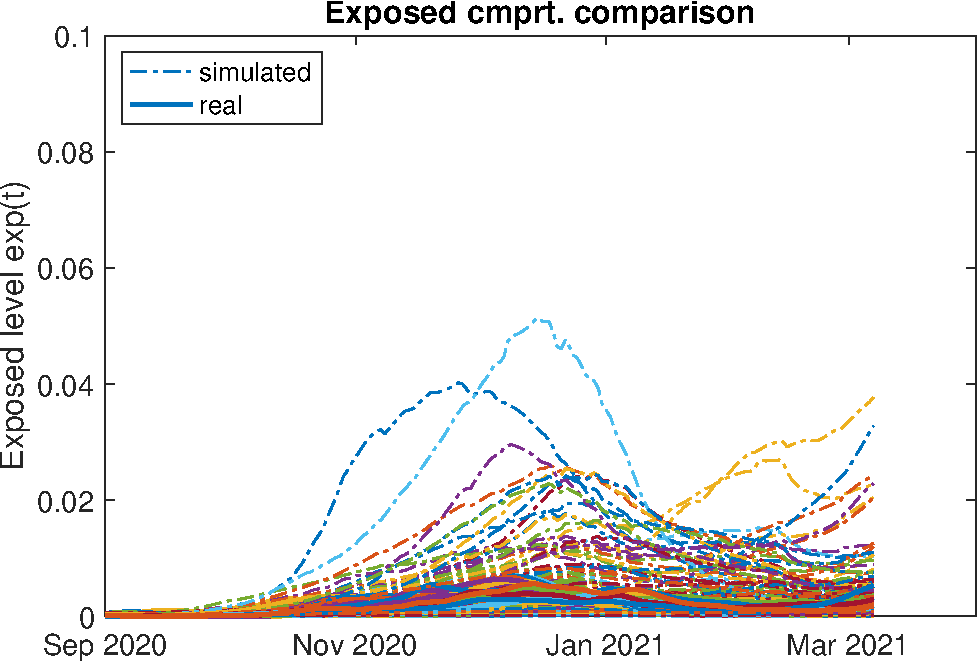
\includegraphics[width=\linewidth]{img/210907_223108_combined_wave2/figures/SEIR_e_sim-vs-real}
         \caption{Exposed}
         \label{fig:compCombWave2Exp}
     \end{subfigure}
     \newline
     \begin{subfigure}[b]{.45\linewidth}
         \centering
         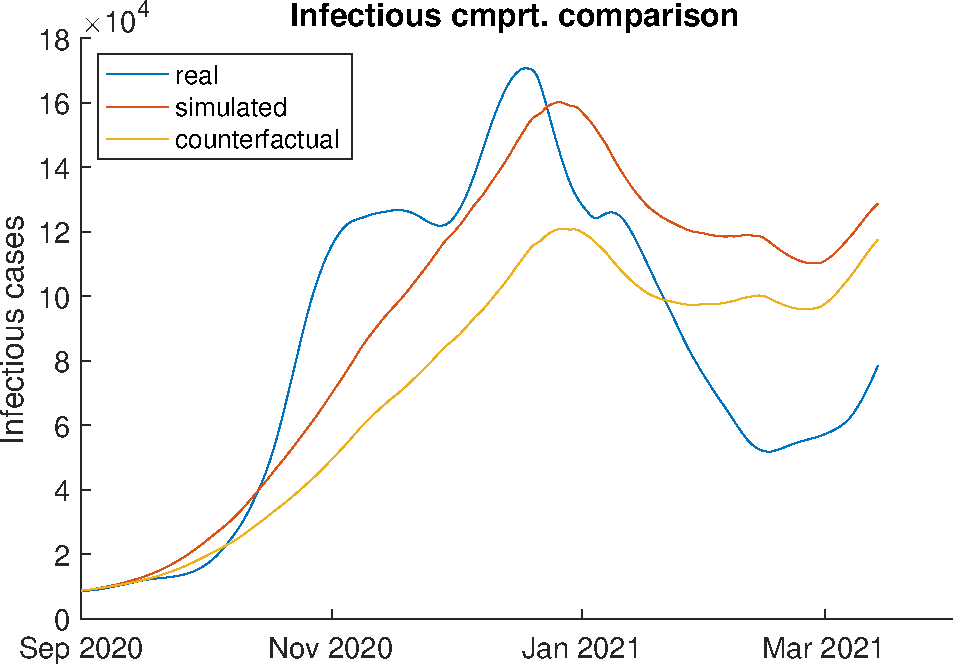
\includegraphics[width=\linewidth]{img/210907_223108_combined_wave2/figures/COMP_inf}
         \caption{Infectious}
         \label{fig:compAggrCombWave2Inf}
     \end{subfigure}
     \hfill
     \begin{subfigure}[b]{.45\linewidth}
         \centering
         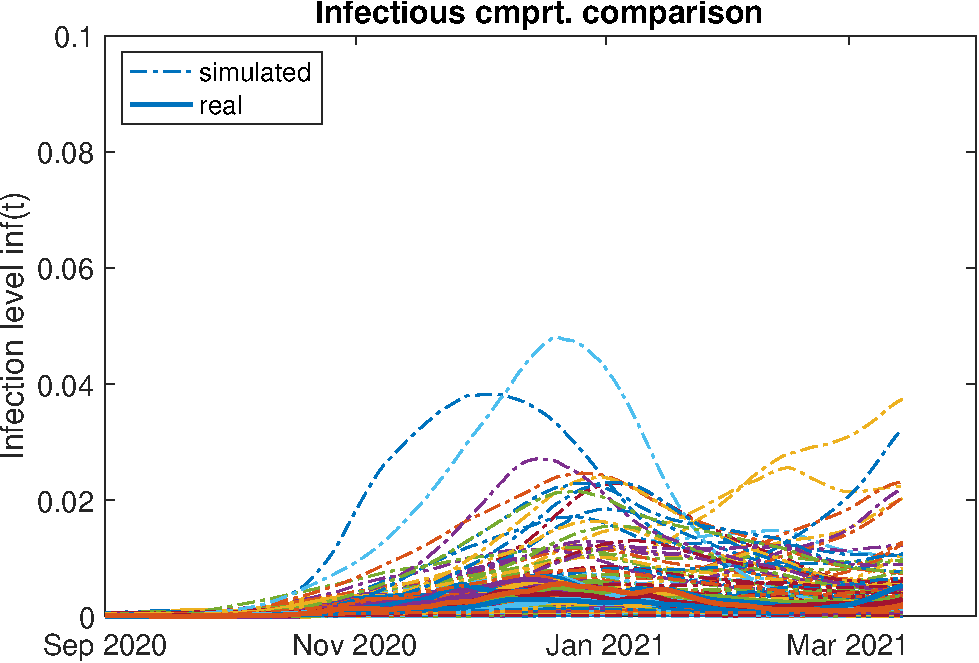
\includegraphics[width=\linewidth]{img/210907_223108_combined_wave2/figures/SEIR_i_sim-vs-real}
         \caption{Infectious}
         \label{fig:compCombWave2Inf}
     \end{subfigure}
     \newline
     \begin{subfigure}[b]{.45\linewidth}
         \centering
         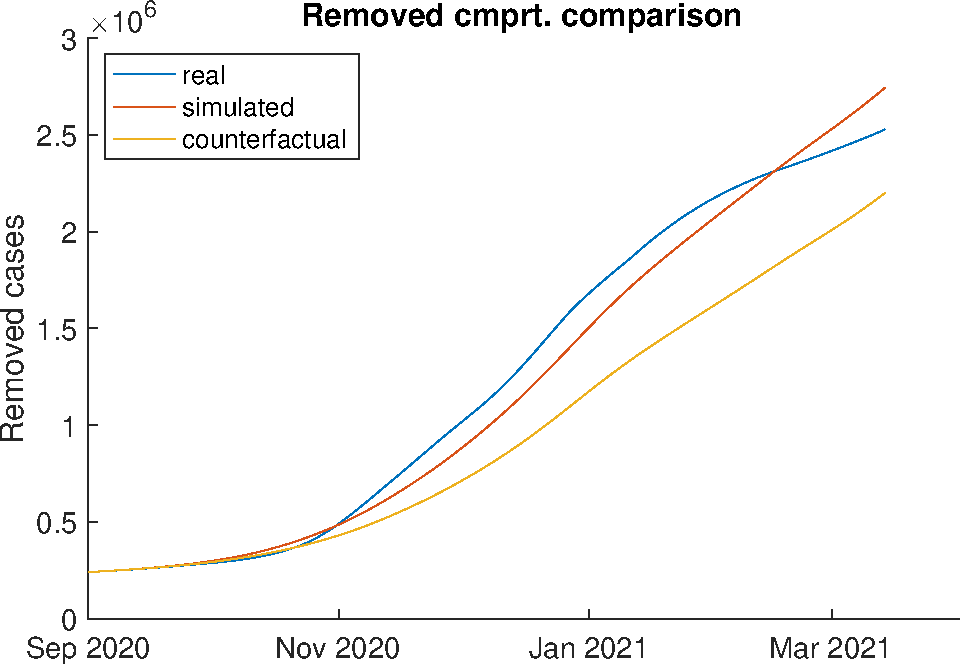
\includegraphics[width=\linewidth]{img/210907_223108_combined_wave2/figures/COMP_rem}
         \caption{Removed}
         \label{fig:compAggrCombWave2Rem}
     \end{subfigure}
     \hfill
     \begin{subfigure}[b]{.45\linewidth}
         \centering
         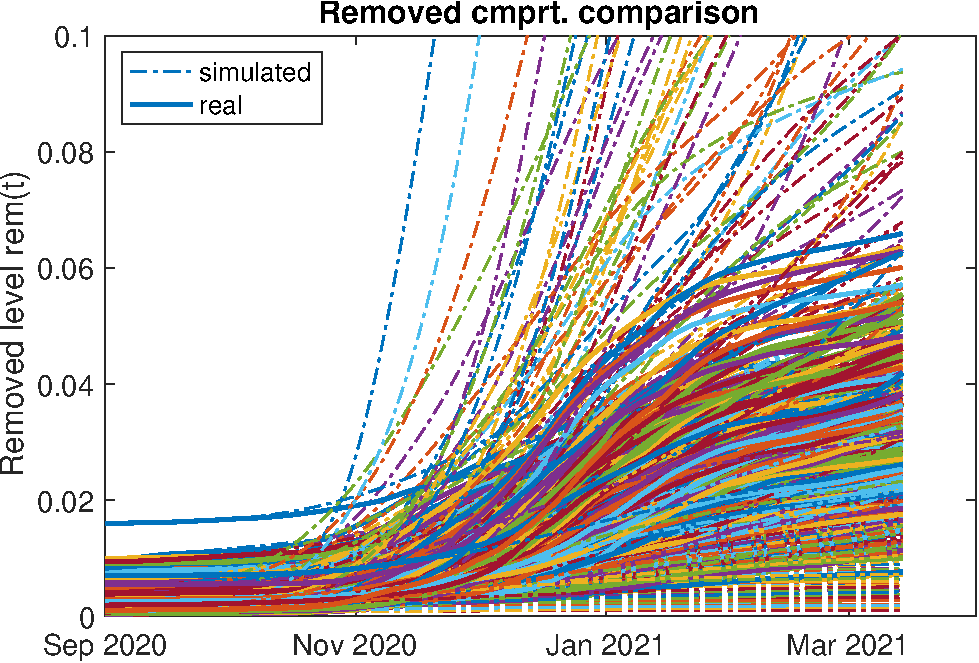
\includegraphics[width=\linewidth]{img/210907_223108_combined_wave2/figures/SEIR_r_sim-vs-real}
         \caption{Removed}
         \label{fig:compCombWave2Rem}
     \end{subfigure}     
     \caption{Compartment levels, wave 2 with combined mobility; left: normalized per county, right: aggregated denormalized}
     \label{fig:compCombWave2}
\end{figure}

\subsection{Wave 3 - from 15-MAR-2021 to 23-JUN-2021}

The analysis of the third wave in \autoref{fig:compCombWave3} is a powerful example for the shortcomings of the approach. The plots clearly show that the simulation is not able to match the actual, measured spread activity and instead predicts an almost constant level of infections--though yielding similar removed compartment levels. This suggests to consider a new compartment for vaccinated cases, as the observed decline of real cases likely results from a decrease in the susceptible compartment due to the success of the vaccination program.

\begin{figure}[hbtp]
     \centering
     \begin{subfigure}[b]{.45\linewidth}
         \centering
         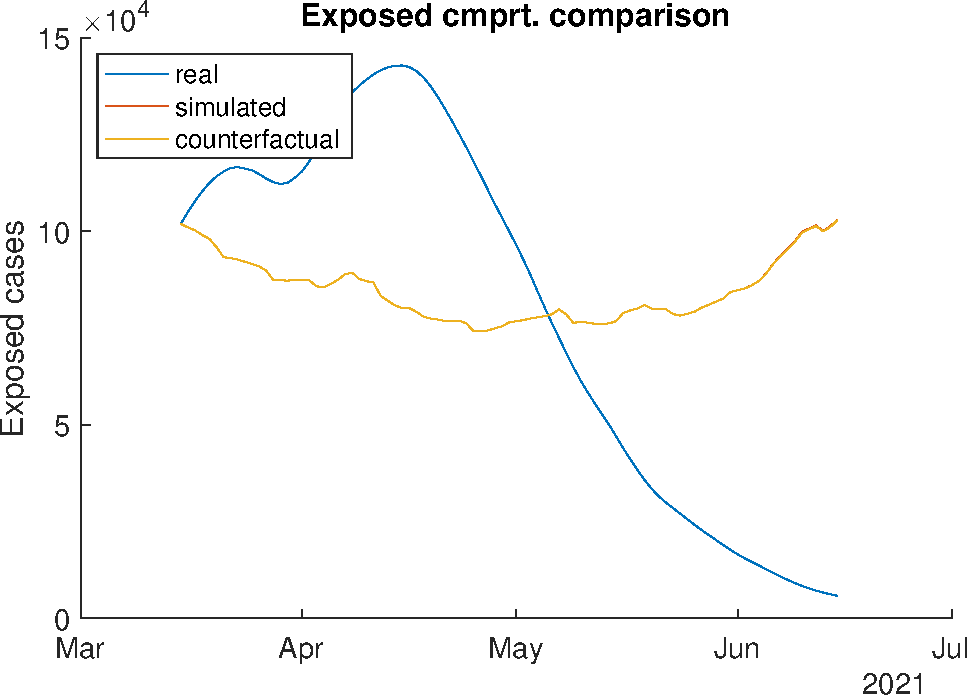
\includegraphics[width=\linewidth]{img/210907_224100_combined_wave3/figures/COMP_exp}
         \caption{Exposed}
         \label{fig:compAggrCombWave3Exp}
     \end{subfigure}
     \hfill
     \begin{subfigure}[b]{.45\linewidth}
         \centering
         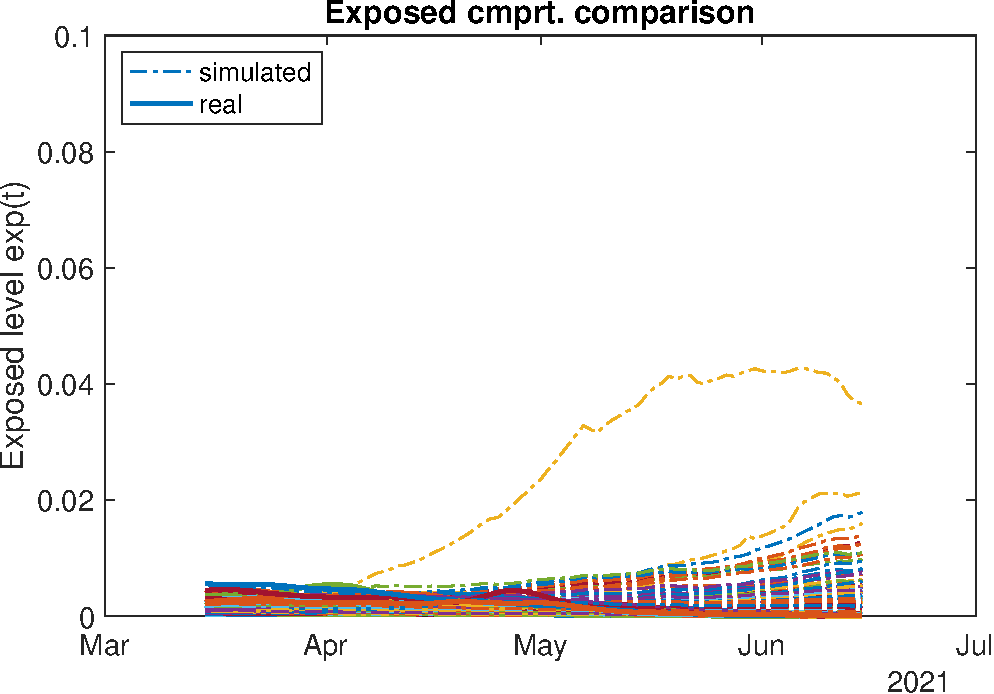
\includegraphics[width=\linewidth]{img/210907_224100_combined_wave3/figures/SEIR_e_sim-vs-real}
         \caption{Exposed}
         \label{fig:compCombWave3Exp}
     \end{subfigure}
     \newline
     \begin{subfigure}[b]{.45\linewidth}
         \centering
         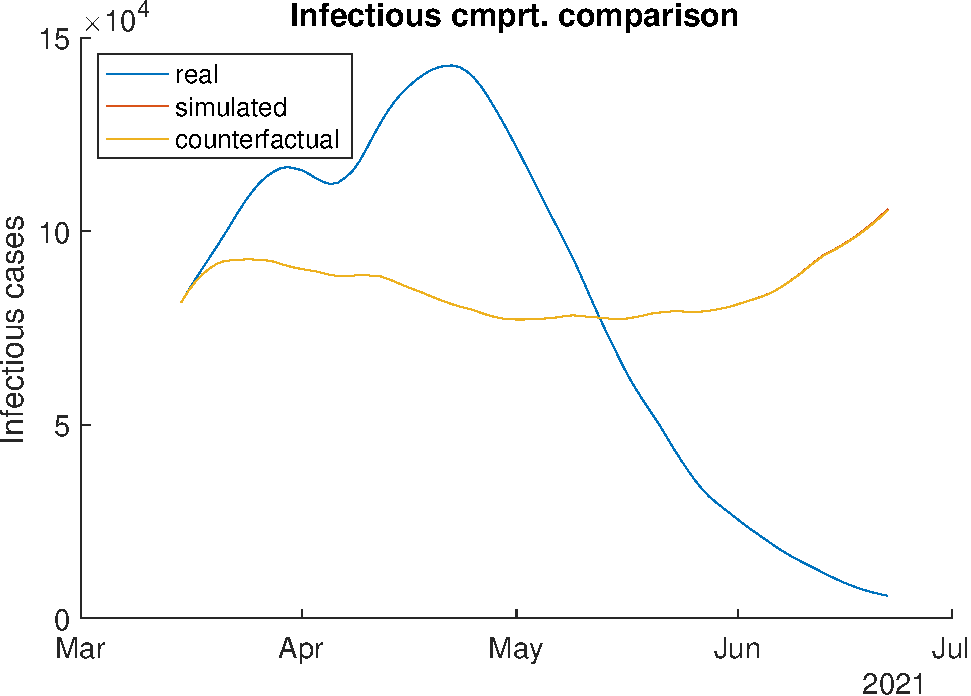
\includegraphics[width=\linewidth]{img/210907_224100_combined_wave3/figures/COMP_inf}
         \caption{Infectious}
         \label{fig:compAggrCombWave3Inf}
     \end{subfigure}
     \hfill
     \begin{subfigure}[b]{.45\linewidth}
         \centering
         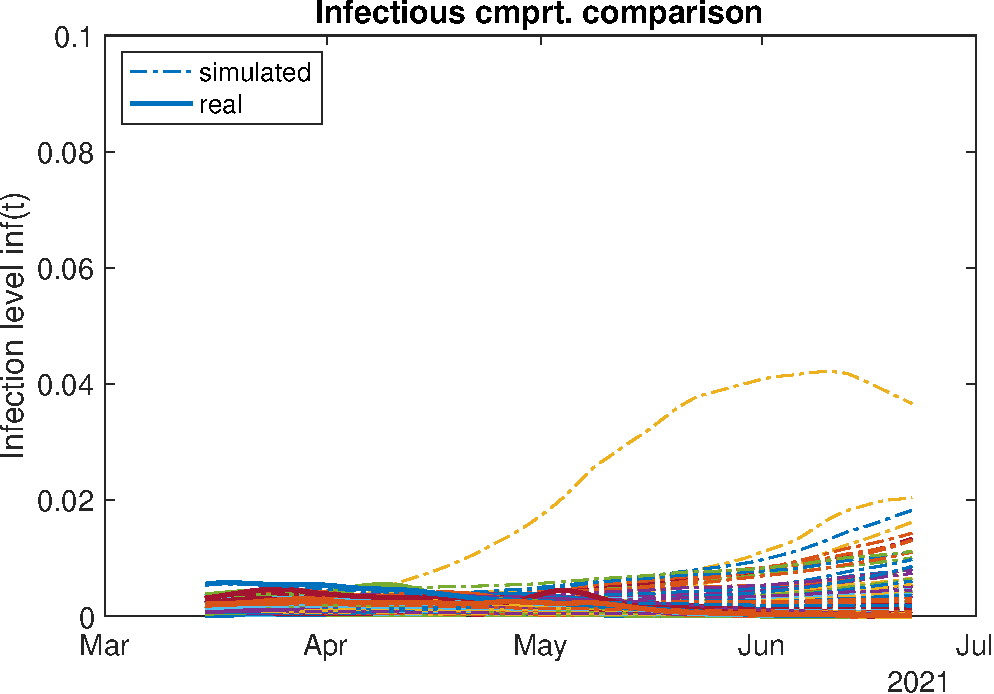
\includegraphics[width=\linewidth]{img/210907_224100_combined_wave3/figures/SEIR_i_sim-vs-real}
         \caption{Infectious}
         \label{fig:compCombWave3Inf}
     \end{subfigure}
     \newline
     \begin{subfigure}[b]{.45\linewidth}
         \centering
         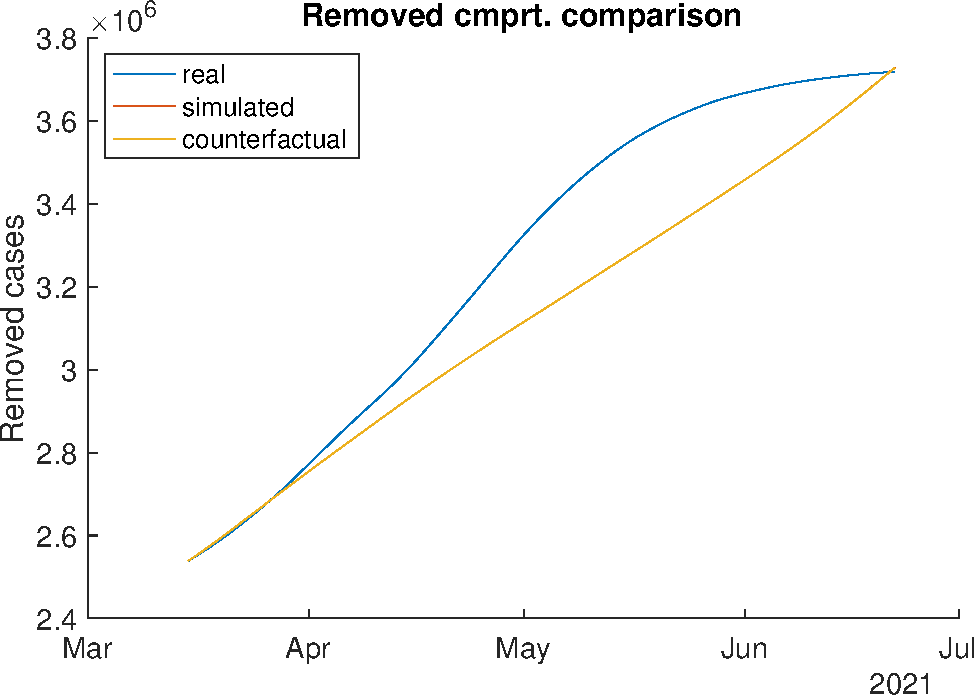
\includegraphics[width=\linewidth]{img/210907_224100_combined_wave3/figures/COMP_rem}
         \caption{Removed}
         \label{fig:compAggrCombWave3Rem}
     \end{subfigure}
     \hfill
     \begin{subfigure}[b]{.45\linewidth}
         \centering
         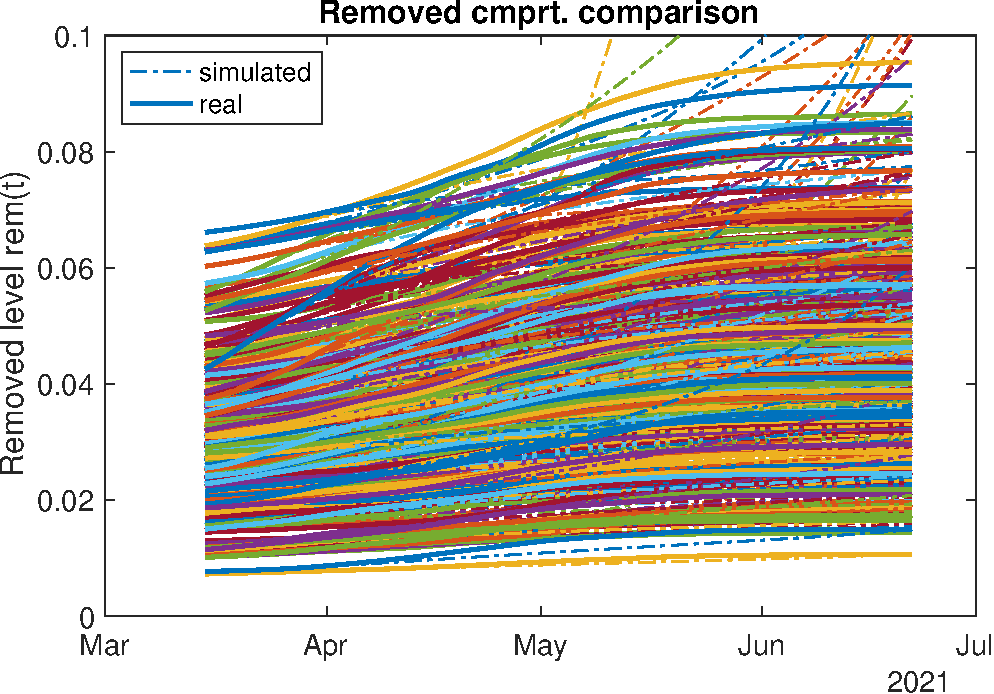
\includegraphics[width=\linewidth]{img/210907_224100_combined_wave3/figures/SEIR_r_sim-vs-real}
         \caption{Removed}
         \label{fig:compCombWave3Rem}
     \end{subfigure}     
     \caption{Compartment levels, wave 3 with combined mobility; left: normalized per county, right: aggregated denormalized}
     \label{fig:compCombWave3}
\end{figure}

\subsection{Waves 2 and 3 - from 01-SEP-2021 to 23-JUN-2021}

The combined analysis of the second and third wave in \autoref{fig:compCombWave23} shows a similar behavior as presented in \autoref{sec:evaluation} except for the huge deviations fore the omitted first wave. The plots support the networked SEIR model's ability to recover the two distinct waves purely from the measured mobility behavior of the population under analysis.

\begin{figure}[hbtp]
     \centering
     \begin{subfigure}[b]{.45\linewidth}
         \centering
         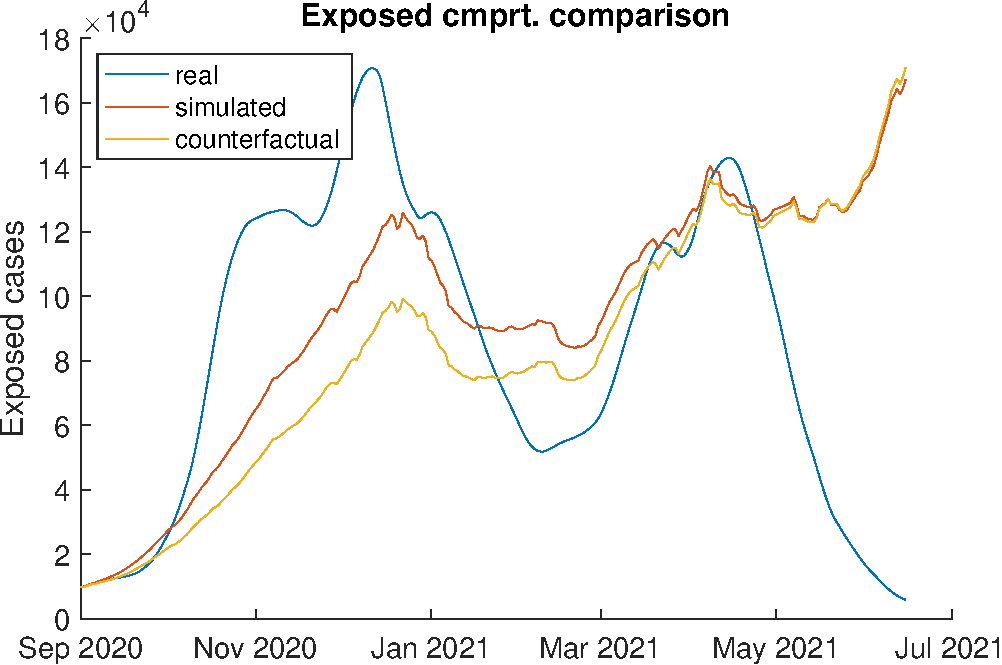
\includegraphics[width=\linewidth]{img/210907_224622_combined_wave23/figures/COMP_exp}
         \caption{Exposed}
         \label{fig:compAggrCombWave23Exp}
     \end{subfigure}
     \hfill
     \begin{subfigure}[b]{.45\linewidth}
         \centering
         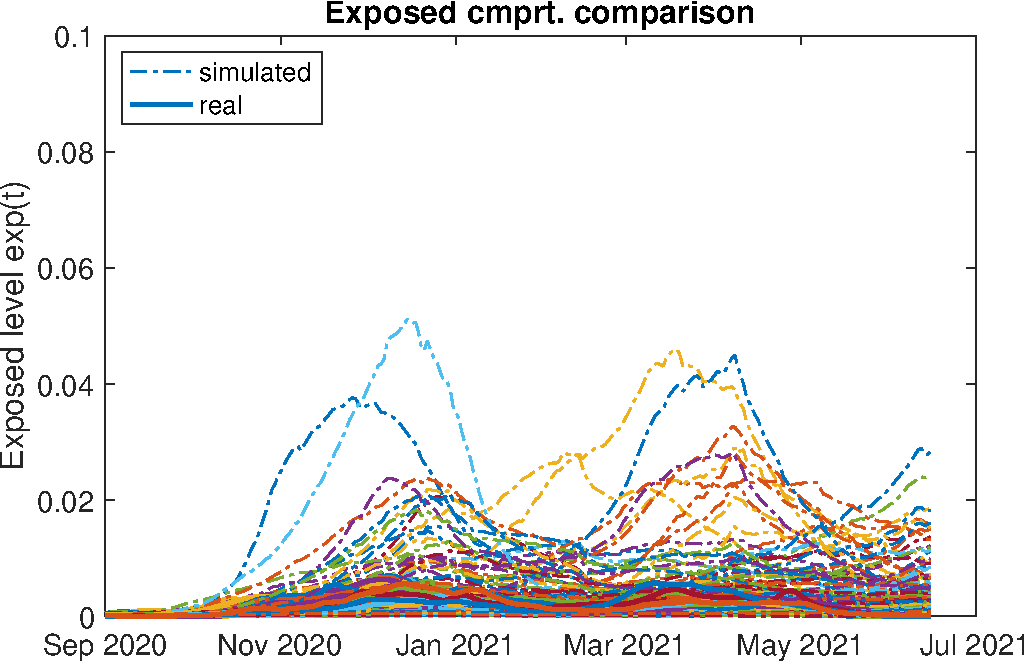
\includegraphics[width=\linewidth]{img/210907_224622_combined_wave23/figures/SEIR_e_sim-vs-real}
         \caption{Exposed}
         \label{fig:compCombWave23Exp}
     \end{subfigure}
     \newline
     \begin{subfigure}[b]{.45\linewidth}
         \centering
         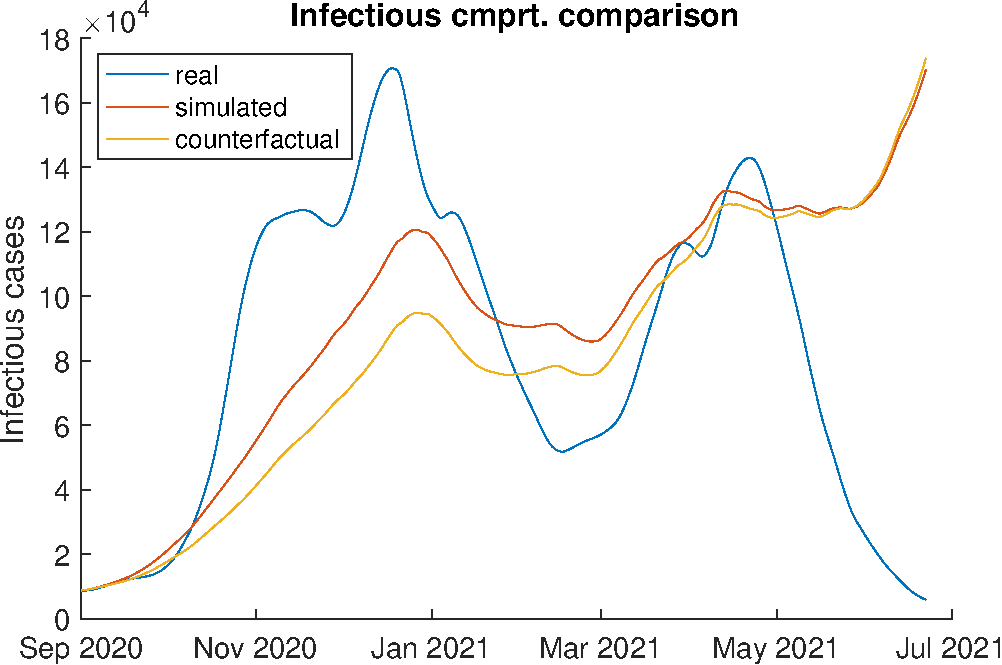
\includegraphics[width=\linewidth]{img/210907_224622_combined_wave23/figures/COMP_inf}
         \caption{Infectious}
         \label{fig:compAggrCombWave23Inf}
     \end{subfigure}
     \hfill
     \begin{subfigure}[b]{.45\linewidth}
         \centering
         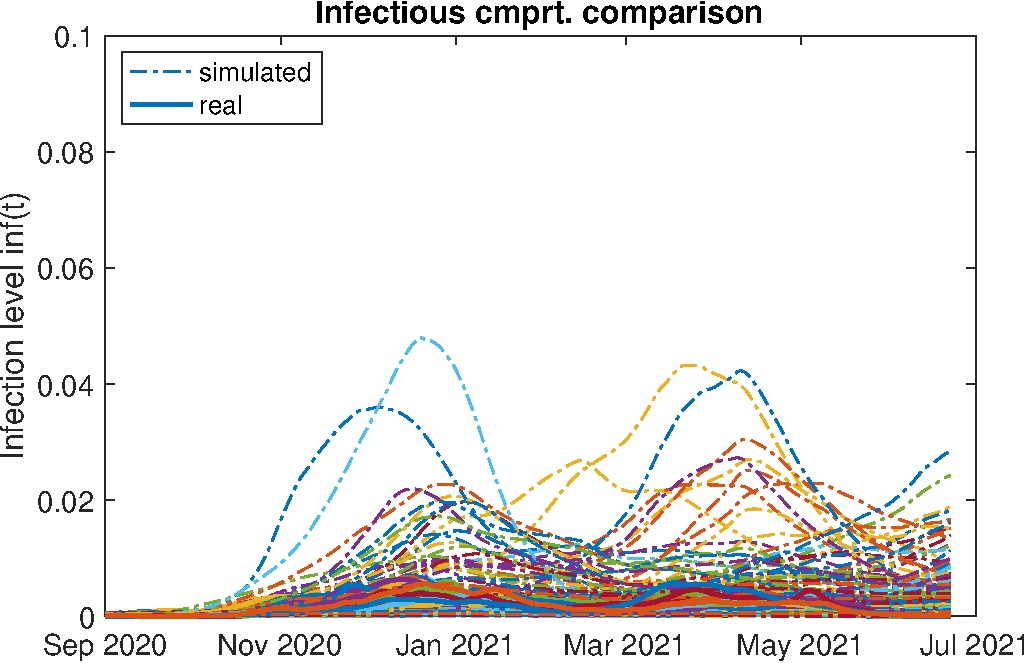
\includegraphics[width=\linewidth]{img/210907_224622_combined_wave23/figures/SEIR_i_sim-vs-real}
         \caption{Infectious}
         \label{fig:compCombWave23Inf}
     \end{subfigure}
     \newline
     \begin{subfigure}[b]{.45\linewidth}
         \centering
         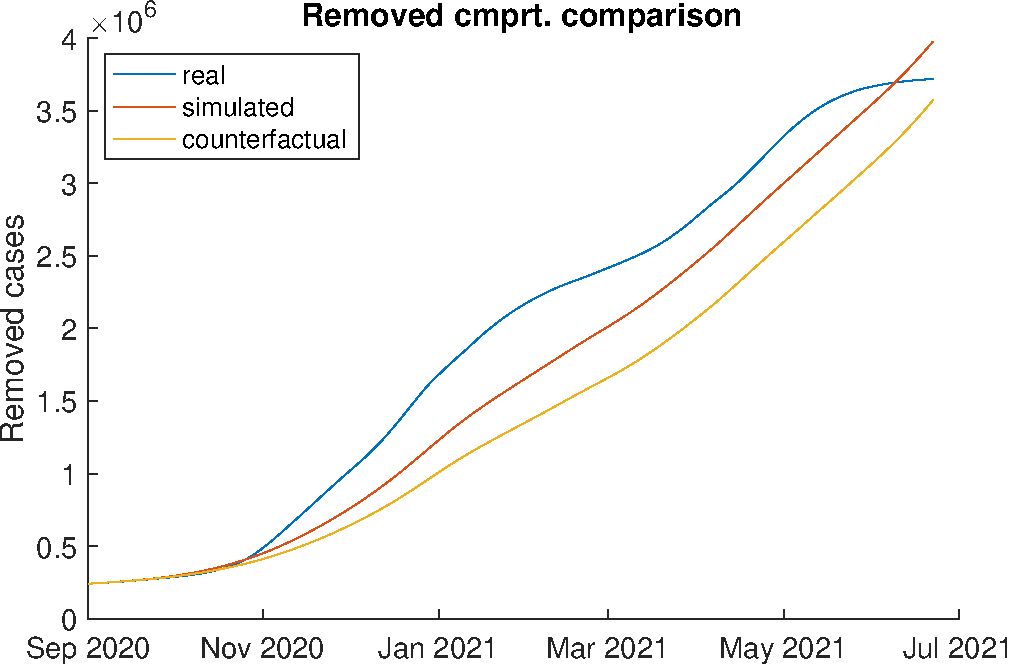
\includegraphics[width=\linewidth]{img/210907_224622_combined_wave23/figures/COMP_rem}
         \caption{Removed}
         \label{fig:compAggrCombWave23Rem}
     \end{subfigure}
     \hfill
     \begin{subfigure}[b]{.45\linewidth}
         \centering
         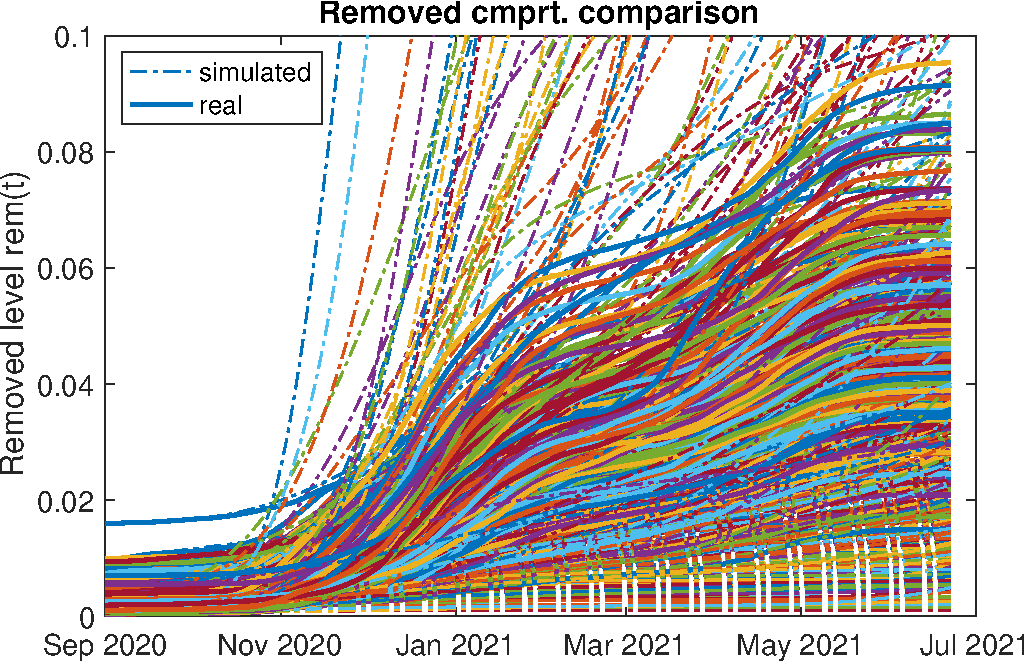
\includegraphics[width=\linewidth]{img/210907_224622_combined_wave23/figures/SEIR_r_sim-vs-real}
         \caption{Removed}
         \label{fig:compCombWave23Rem}
     \end{subfigure}     
     \caption{Compartment levels, waves 2\&3 with combined mobility; left: normalized per county, right: aggregated denormalized}
     \label{fig:compCombWave23}
\end{figure}

\section{Data sets and formats}
This section introduces specialties and caveats about the data sets used in the report and how their specific formats work. The interested reader is guided to other resources for further reading. The data sets are aggregated and made available in their raw form in the following public git repository free of charge using the git LFS technology: \url{https://github.com/hashkode/covid-data}

\subsection{Mobility data - GTFS}
The mobility data used herein is provided by the DELFI e.V. and licensed under \href{https://creativecommons.org/licenses/by/4.0/deed.de}{CC BY 4.0}.\cite{delfie.v.OpenDataOPNV2021}
The data set is provided in the format of GTFS, which is a standardized format originating from Google. The reference documentation for the format describing all involved files, keys and possible uses can be found here: \href{https://developers.google.com/transit/gtfs/reference}{GTFS Reference}.

\subsection{COVID-19 data - RKI}
The COVID-19 data used in this project is taken from the Robert Koch-Institut (RKI). It consists of:
\begin{itemize}
	\item Daily caseload per age group, gender and county for Germany in the form of a timetable \cite{robertkoch-institutrkiRKICOVID192021} licensed under \href{https://www.govdata.de/dl-de/by-2-0}{DL-DE/BY-2.0} and
	\item daily vaccination information on a national and state level \cite{robertkoch-institutrkiRKICoronavirusSARSCoV22021} also licensed under \href{https://www.govdata.de/dl-de/by-2-0}{DL-DE/BY-2.0}.
\end{itemize}

\subsection{Mobility behavior data - DESTATIS}
The mobility data that is used to prepare the behavior vector mentioned in \eqref{eq:6a}, \eqref{eq:6b} and \eqref{eq:6c} is provided by the German Statistics Office named DESTATIS. Two different data sets are used herein:
\begin{itemize}
	\item Relative change in total mobility behavior compared to 2019 levels per county as a timetable \cite{statistischesbundesamtdestatisVeranderungsrateMobilitatGgu2021} licensed for free use with reference \href{https://www.destatis.de/DE/Service/Impressum/copyright-allgemein.html}{DESTATIS - Copyright allgemein} and
	\item Relative change mobility behavior for different modes of travel compared to 2019 levels aggregated on the national level as a timetable \cite{statistischesbundesamtdestatisVerkehrsmittelImFernverkehr2021} licensed for free use with reference \href{https://www.destatis.de/DE/Service/Impressum/copyright-allgemein.html}{DESTATIS - Copyright allgemein}.
\end{itemize}
